\documentclass[12pt,a4paper]{article}
\usepackage{graphicx} % Required for inserting images
\usepackage{ucs}
\usepackage{float}
\usepackage[utf8x]{inputenc}
\usepackage[russian]{babel}
\usepackage{hyphenat}
\usepackage{amsmath}
\usepackage{tabularx} 
\usepackage{adjustbox} 
\usepackage{makecell} 
\usepackage{listings}
\usepackage{xcolor}
\usepackage{enumitem}
\usepackage{pgfplotstable}
\usepackage{graphicx}
\usepackage{pgfplots}
\usepackage{colortbl}
%\usepackage{../lecture-notes/vkCourseML}
%\usepackage{lipsum}
%\usepackage{indentfirst}
\title{Машинное обучение, ФКН ВШЭ\\Семинар №6}
\author{}
\date{}
\begin{document}

\maketitle
\section{Предсказание вероятностей}

\par Задача прогнозирования вероятностей относится к \textit{мягкой} классификации. Качество мягкой классификации нельзя корректно измерять метриками жёсткой классификации (accuracy, precision, recall), так как они игнорируют сами вероятности и учитывают только выбранный порог. Также для оценки качества мягкой классификации недостаточно использовать метрики ранжирования, такие как ROC-AUC: они показывают, насколько хорошо модель различает классы при разных порогах, но ничего не говорят о том, насколько правильно откалиброваны вероятности. 

В семинаре разберемся, каким требованиям должен удовлетворять классификатор, чтобы его выход можно было расценивать как оценку вероятности класса.

\subsubsection*{Когда нужны вероятности?}

Вероятности могут быть использованы в различных сценариях. Например, в случае взаимодействия с продуктом, на основе вероятностей можно группировать клиентов и взаимодействовать с ними разными стратегиями, основываюсь на вероятности целевого действия. Числовой пример — если модель $\hat{p}(x)$ откалибрована, то ожидаемый доход от клиента $x$, который потратит $f(x)$ при покупке, можно рассчитать как $\hat{p}(x) f(x)$. В этом случае оптимальная стратегия — звонить клиентам с наибольшим ожидаемым доходом. И стратегия окажется проигрышной, если вероятности не имеют ничего общего с реальностью.  


\subsubsection*{Откаблиброванная модель.}

Пусть задана выборка $X$. Модель $\hat{p}(x)$ будем называть \textbf{откалиброванной}, если среди всех объектов $x' \in X$, для которых $\hat{p}(y=1| x') = k$, $k \in [0, 1]$, ровно $k\cdot100\%$ процентов действительно принадлежат целевому классу. 


%\par Пусть в каждой точке $x \in \mathbb{X}$ пространства объектов
%задана вероятность~$p(y=+1 \cond x)$ того, что данный объект относится
%к классу $+1$, и пусть алгоритм~$b(x)$ возвращает числа из отрезка~$[0, 1]$. Потребуем, чтобы эти предсказания пытались в каждой точке~$x$ приблизить вероятность положительного класса~$p(y = +1 | x)$.
\par Выполнение этого требования зависит от функции потерь ~---
минимум ее матожидания в каждой точке $x$ должен достигаться на данной вероятности:
$$\arg \min_{\hat{p}\in \mathbb{R}} \mathbb{E} \left[ L(y, \hat{p(x)})|x \right] = p(y=+1|x).$$

где $p(y=+1|x)$ — истинная вероятность. Для краткости изложения, обозначим спрогнозированную вероятность в точке $x$ как $\hat{p}.$ На примере двух функций потерь рассмотрим, как именно связана идеальная вероятность и минимизация функции. 

\subsubsection*{Задача 1.} 
Показать, что квадратичная функция потерь $$L(y, \hat{p}) = ([y = +1] - \hat{p})^2$$
 позволяет предсказывать корректные вероятности. \\

% b to \hat{p}
\textbf{Решение.} 
Как прежде, обозначим за $p(y=+1|x)$ истинную вероятность объекта принадлежать классу 1 при условии $x$. Заметим, что поскольку алгоритм возвращает числа от 0 до 1, то его ответ должен быть близок к единице, если объект относится к положительному классу, и к нулю~--- если объект относится к отрицательному классу.

Так как  $y \in \{0, 1\}$, то её полное матожидание есть $$\mathbb{E} \left[ L(y, \hat{p})|x\right] =\sum_{y_i \in \{0, 1\}} p(y=y_i|x)L(y, \hat{p}),$$ что эквивалентно:

$$\mathbb{E} \left[ L(y, \hat{p})|x\right] = p(y=1|x)(\hat{p}-1)^2 + (1-p(y=1|x))(\hat{p}-1)^2.$$

Продифференцируем по~$\hat{p}$:

$$\frac{\partial}{\partial \hat{p}} \mathbb{E} \left[L(y, \hat{p})|x \right] = 2p(y = 1 | x) (\hat{p} - 1) + 2(1 - p(y = 1 | x))\hat{p}
	=
	2\hat{p} - 2p(y = 1 | x)
	=
	0.$$
	Легко видеть, что оптимальный ответ алгоритма действительно
	равен вероятности:
	$$\hat{p} = p(y = +1 | x).$$


\subsubsection*{Задача 2.} Показать, что абсолютная функция потерь~$L(y, \hat{p}) = |[y = 1] - \hat{p}|, \, \hat{p} \in [0; 1],$ не позволяет предсказывать корректные вероятности.

\textbf{Решение.} \\

Запишем матожидание функции потерь в точке~$x$:
\begin{align*}
		\mathbb{E} \left[ L(y, \hat{p})|x\right] = &p(y=1|x)|1-\hat{p}| + (1 - p(y=1|x))|\hat{p}| = \\
		&= p(y=1|x)(1-\hat{p})+ (1 - p(y=1|x))\hat{p}.\\
\end{align*}

Продифференцируем по~$\hat{p}$:
	$$\frac{\partial}{\partial \hat{p}}
	\mathbb{E} \left[
	L(y, \hat{p})
	|
	x
	\right] =
	1 - 2 p(y = 1 | x) = 0.$$
Рассмотрим 2 случая:

\begin{enumerate}
		\item $p(y=+1|x) = \frac{1}{2}.$ Тогда $\mathbb{E} \left[ L(y, \hat{p})|x\right] = \frac{1}{2} \quad \forall \hat{p} \in [0; 1],$ а потому классификатор не позволяет предсказывать корректную вероятность в точке $x$.
		\item $p(y=+1|x) \ne \frac{1}{2}.$ В этом случае интервал $(0; 1)$ не содержит критических точек, а потому минимум матожидания достигается на одном из концов отрезка $[0; 1]:$
		\begin{align*}
			\min_{\hat{p} \in [0;1]} \mathbb{E} \left[ L(y, \hat{p})|x\right] = 
			\min \left(\mathbb{E} \left[ L(y, 0)|x\right], \mathbb{E} \left[ L(y, 1)|x\right] \right) =\\
			\min \left(p(y = +1 | x), 1 - p(y = +1 | x)\right).
		\end{align*}
		Отсюда $\arg \min_{\hat{p}\in [0;1]} \mathbb{E} \left[ L(y, b)|x\right] \in \{0, 1\},$ а потому классификатор также не позволяет предсказывать корректную вероятность в точке $x$.
	\end{enumerate}
\end{esSolution}

\section{Калибровка вероятностей}

Чтобы получить откалиброванную модель, необходимо в общем случае сделать надстройку над моделью (новую модель), которая получает на вход вероятность, спрогнозированную исходным классификатором $\hat{p}(x)$ и переводит её в вероятность более \textbf{близкую к эмпирической}.  

Универсального критерия, являющегося индикатором откалиброванной модели нет. Однако  сравнить качество вероятностей в двух моделях позволяют квадратичная (она же Brier Score) и логистическая функции потерь. 

$$
LogLoss = -\frac{1}{n}\sum_{i=1}^n \Big(y_i \log p_i + (1-y_i)\log (1-p_i)\Big),
$$

\begin{itemize}
    \item В идеальном случае Log Loss равна 0.
    \item В худшем случае Log Loss стремится к $∞$.
\end{itemize} В идеальном случае Log Loss равна 0.

$$
\mbox{BrierScore} = \frac{1}{n} \left(\sum_{i} (y_i-p_i)^2 \right)
$$

\begin{itemize}
    \item В худшем случае Brier score равна 1. 
    \item В лучше случае Brier score $\to$ 0. 
\end{itemize}

Другим способом оценки вероятностей является калибровочная кривая. На этой кривой абсцисса точки соответствуют значению $p$ (предсказаний алгоритма), а ордината соответствует доле положительных примеров, для которых алгоритм предсказал вероятность, близкую к $p$. В идеальном случае эта кривая совпадает с прямой $y = x$. Примеры такой общего вида кривых для разных алгоритмов приведены на рис. (\ref{fig:plot}).
Изучим два стандартных метода для калибровки вероятностей алгоритма: калибровка Платта и изотоническая регрессия.


\begin{center}
\begin{figure}[!ht]
\centering
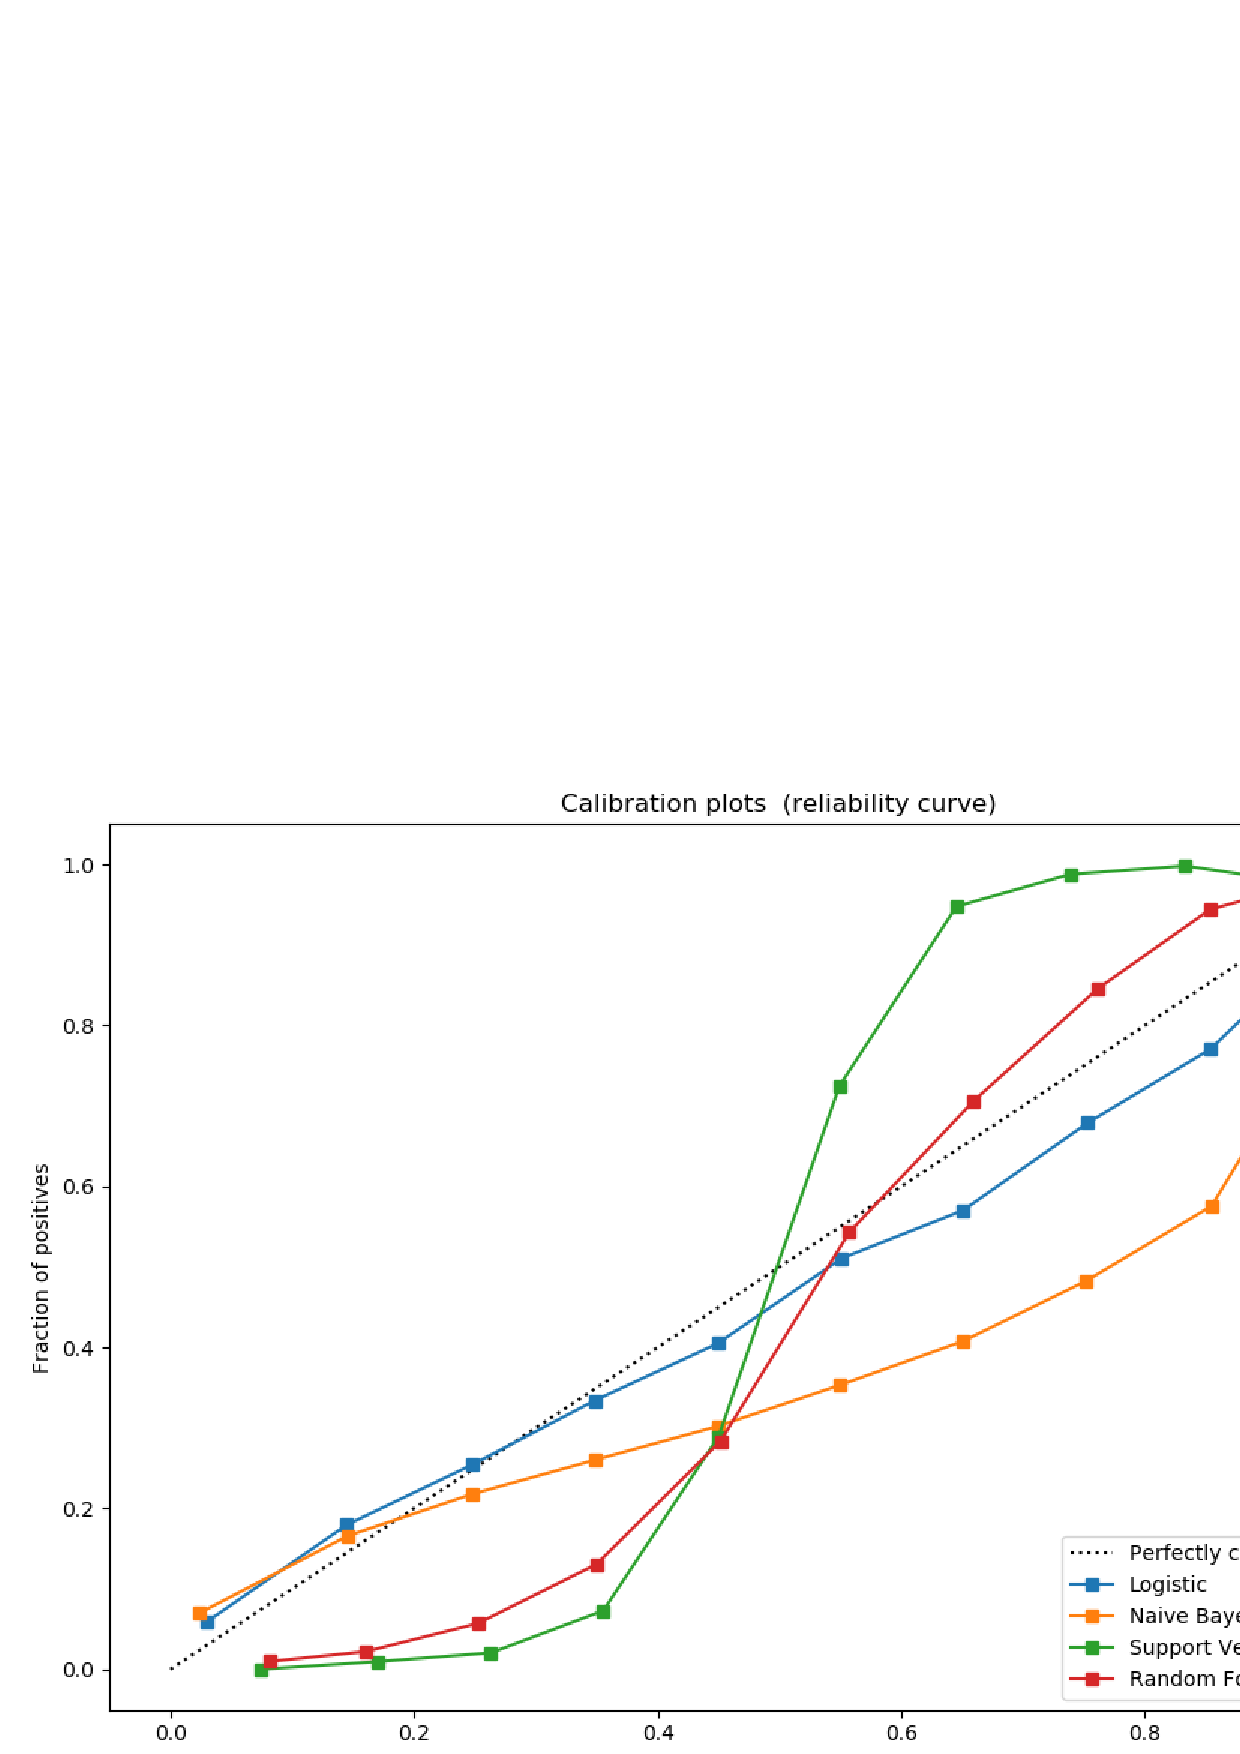
\includegraphics[width=1\linewidth]{img/calibration_plot.png}
\caption{Калибровочные кривые нескольких алгоритмов}\label{fig:plot}
\end{figure}
\end{center}

\subsection{Калибровка Платта}

Пусть наш алгоритм выдаёт значения $f(x)$ (могут не быть вероятностями). Тогда итоговая вероятность:

$$P(y = 1 | x) = \frac{1}{1+\exp (af(x) + b)},$$

где $a, b$ -- скалярные параметры. Эти параметры настраиваются методом максимума правдоподобия (минимизируя логистическую функцию потерь) на отложенной выборке или с помощью кросс валидации. Также Платт предложил настраивать параметры на обучающей выборке базовой модели, а для избежания переобучения изменить метки объектов на следующие значения:

$$t_{+} = \frac{N_{+} + 1}{N_{-} + 2}$$ для положительных примеров и

$$t_{-} = \frac{1}{N_{-} + 2}$$ для отрицательных.

Калибровку Платта можно представить как применения логистической регрессии поверх предсказаний другого алгоритма с отключенной регуляризацией.


\subsection{Изотоническая регрессия}

В этом методе также строится отображение из предсказаний модели в откалиброванные вероятности. Для этого используем изотоническую функцию (неубывающая кусочно-постоянная функция), в которой $x$ -- выходы нашего алгоритма, а $y$ -- целевая переменная. Иллюстрация изотонической регрессии на рис. (\ref{fig:isotonic}).

Мы хотим найти такую функцию $m(t)$: $P(y = 1 | x) = m(f(x))$. Она настраивается под квадратичную ошибку:

$$m = \argmin_{z} \sum (y_i - z(f(x_i))^2,$$

с помощью специального алгоритма (Pool-Adjacent-Violators Algorithm), изучать который в этом курса не будем.

\begin{center}
\begin{figure}[!htb]
\centering
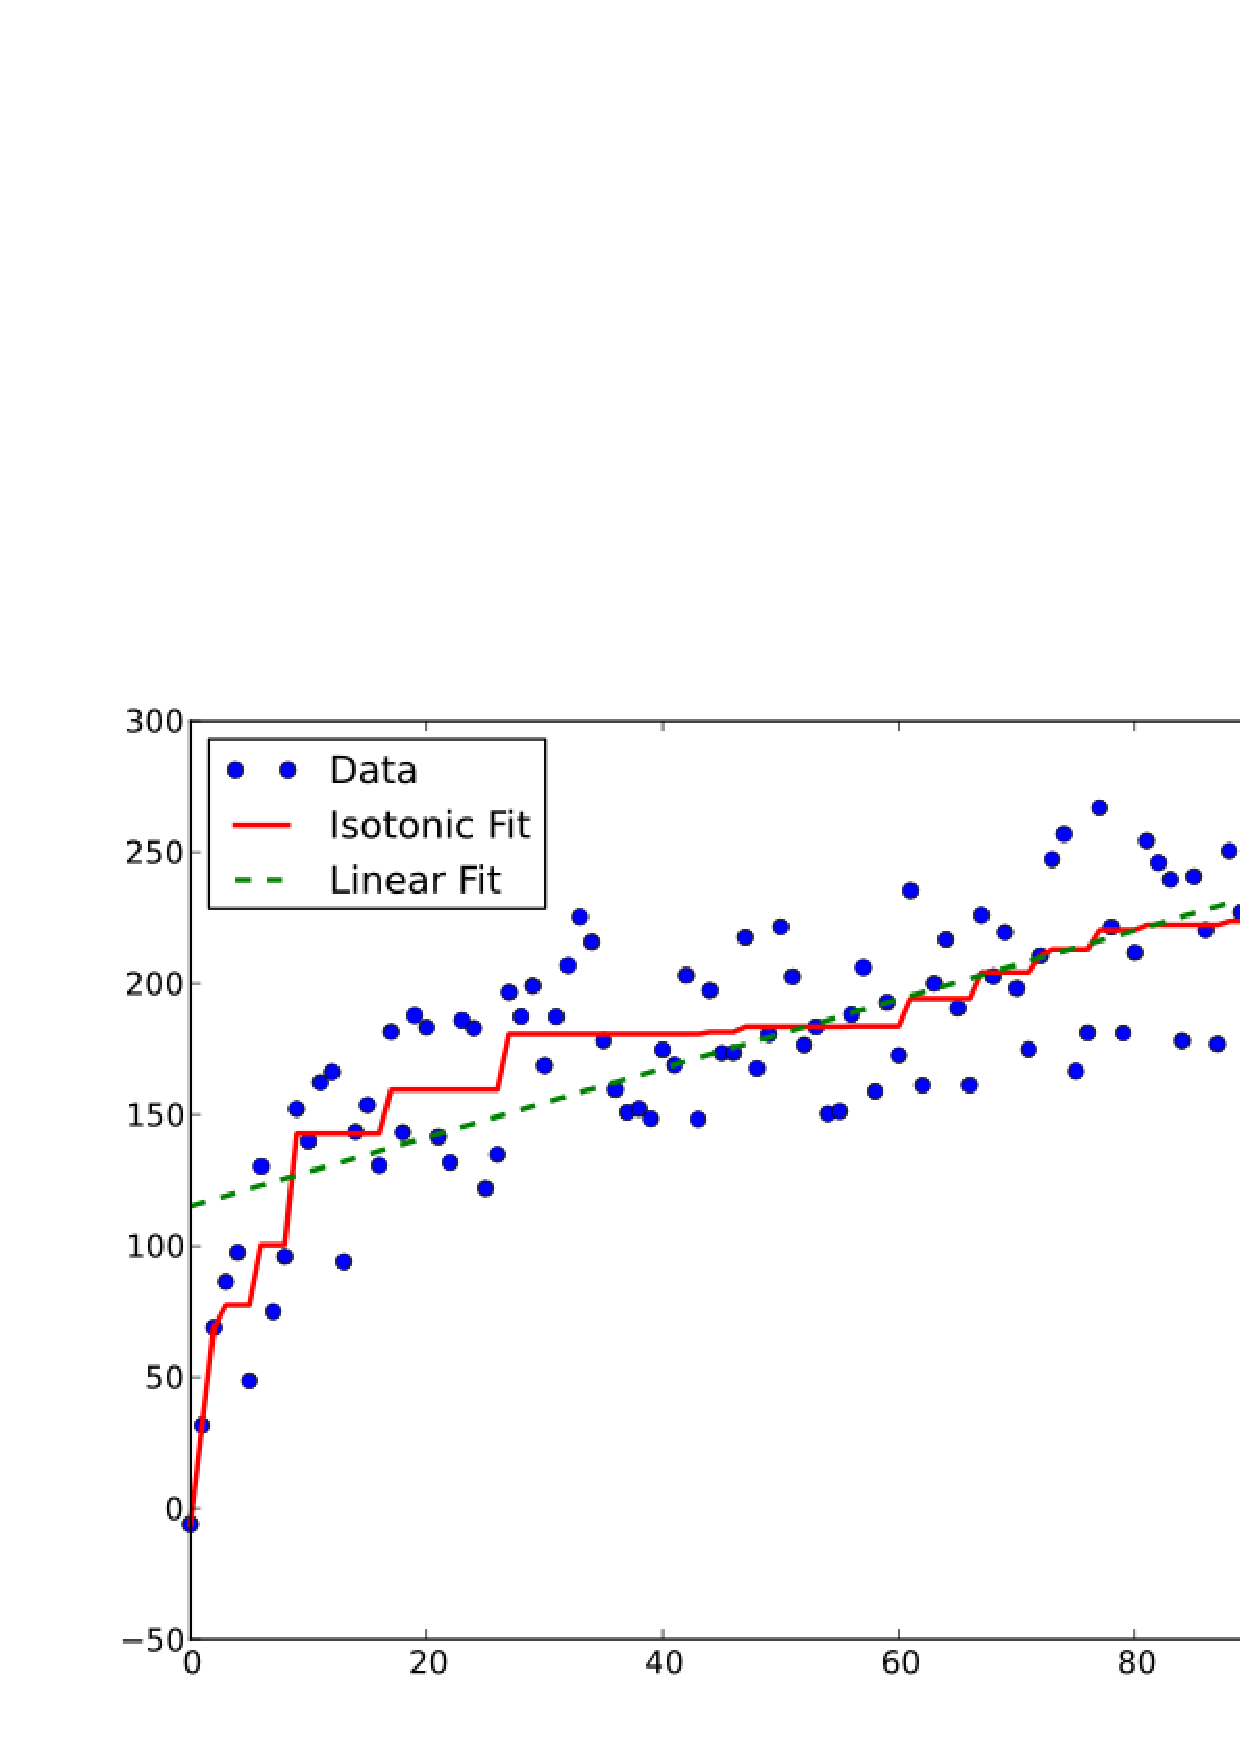
\includegraphics[width=1\linewidth]{img/isotonic.png}
\caption{Изотоническая регрессия}\label{fig:isotonic}
\end{figure}
\end{center}


В результате калибровки получаем надстройку над нашей моделью, которая применяется поверх предсказаний базовой модели. В случае мультиклассовой классификации каждый класс калибруется отдельно против остальных (one-versus-all), вероятности при предсказании нормируются.


\subsection{Квантильная регрессия}

В некоторых задачах цены занижения и завышения прогнозов могут отличаться друг от друга.
Например, при прогнозировании спроса на товары интернет-магазина гораздо опаснее заниженные
предсказания, поскольку они могут привести к потере клиентов.
Завышенные же прогнозы приводят лишь к издержкам на хранение товара на складе.
Функционал в этом случае можно записать как
\[
    Q(a, X^\ell)
    =
    \sum_{i = 1}^{\ell}
        \rho_\tau(y_i - a(x_i)),
\]
где
\[
    \rho_\tau(z)
    =
    (\tau - 1) [z < 0] z
    +
    \tau [z \geq 0] z
    =
    (\tau - \frac{1}{2})z + \frac{1}{2} |z|,
\]
а параметр~$\tau$ лежит на отрезке~$[0, 1]$ и определяет
соотношение важности занижения и завышения прогноза.
Чем больше здесь~$\tau$, тем выше штраф за занижение прогноза.

Обсудим вероятностный смысл данного функционала.
Будем считать, что в каждой точке~$x \in \XX$ пространства объектов
задано вероятностное распределение~$p(y|x)$ на возможных ответах для данного объекта.
Такое распределение может возникать, например, в задаче предсказания кликов по рекламным баннерам:
один и тот же пользователь может много раз заходить на один и тот же сайт и видеть данный баннер;
при этом некоторые посещения закончатся кликом, а некоторые~--- нет.

Известно, что при оптимизации квадратичного функционала алгоритм~$a(x)$
будет приближать условное матожидание ответа в каждой точке пространства
объектов:~$a(x) \approx \mathbb{E} [y | x]$;
если же оптимизировать среднее абсолютное отклонение, то итоговый алгоритм
будет приближать медиану распределения:~$a(x) \approx \text{median} [p(y | x)]$.
Рассмотрим теперь некоторый объект~$x$ и условное распределение~$p(y | x)$.
Найдем  число~$q$, которое будет оптимальным с точки зрения нашего функционала:
\[
    Q = \int_\YY \rho_\tau(y - q) p(y | x) dy.
\]
Продифференцируем его~(при этом необходимо воспользоваться правилами
дифференцирования интегралов, зависящих от параметра):
\[
    \frac{\partial Q}{\partial q}
    =
    (1 - \tau) \int_{-\infty}^{q} p(y | x) dy
    -
    \tau \int_{q}^{\infty} p(y| x) dy
    =
    0.
\]
Получаем, что
\[
    \frac{\tau}{1 - \tau}
    =
    \frac{
        \int_{-\infty}^{q} p(y \cond x) dy
    }{
        \int_{q}^{\infty} p(y \cond x) dy
    }.
\]
Данное уравнение будет верно, если~$q$ будет равно~$\tau$-квантили распределения~$p(y \cond x)$.
Таким образом, использование функции потерь~$\rho_\tau(z)$ приводит к тому,
что алгоритм~$a(x)$ будет приближать~$\tau$-квантиль распределения ответов в каждой точке
пространства объектов.


\subsection{Beta Calibration}

Beta Calibration — это развитие калибровки Платта. Однако, если в калибровке Платта у нас было 2 параметра, то здесь испольузется 3. 

$$
P(y=1|x) = \left(1+ \frac{1}{\exp(c)\, \frac{f(x)^a}{(1-f(x))^b}} \right)^{-1},
$$

где $f(x)$ — некалиброванная вероятность. В отличие от стандартного логистического преобразования (2 параметра), добавление третьего параметра делает модель гибче и позволяет аппроксимировать широкий класс кривых. Важным свойством является то, что семейство функций включает прямую $y=x$, поэтому если модель уже откалибрована, калибровка не ухудшит результат. Попрактиковаться с данной калибровкой можно, используя код семинара. 

\section{Мультиклассовая калибровка}

В задачах с более чем двумя классами проблема калибровки модифицируется. А именно, теперь нам необходим корректные вероятности для всех категорий, которые должны суммироваться в единицу. Один из подходов к мультиклассовой калибровке — сведение задачи к набору бинарных классификаций с последующим объединением результатов.

Существует несколько стандартных способов разложения многоклассовой задачи на бинарные подзадачи. Базовые:

\begin{itemize}
    \item One-vs-One (all pairs). Для классов $c_1, c_2, ..., c_n$ строим $\frac{n(n-1)}{2}$ классификаторов и калибруем каждый из них.
    \item One-vs-All: для $n$ классов обучаем $n$ классификаторов «один класс против всех остальных».
\end{itemize} 

\begin{center}
\begin{figure}[!ht]
\centering
\includegraphics[width=1\linewidth]{img/one_vs_.png}
\caption{Базовые подходы сведения мультиклассовой задачи к серии бинарных}\label{fig:one_vs}
\end{figure}
\end{center}

Далее, каждую бинарную задачу можно откалибровать любым подходящим методом. После калибровки бинарных задач возникает задача «сбора» вероятностей так, чтобы итоговый вектор вероятностей $$\vec{p} = (p_1, p_2, ..., p_n),$$ был таким, что $p_i \geq 0, \sum_ip_i=1$. 
\newline

В схеме one-vs-all, если $\hat p_i$ — откалиброванная вероятность для задачи «$i$ против всех», то многоклассовую вероятность можно получить нормализацией:

$$ \tilde{p}_i = \frac{\hat{p}_i}{\sum_j \hat{p}_j}.$$

В схеме one-vs-one можно сначала суммировать все вероятности в парах $i-j$ в пользу класса $i$:

$$ \tilde{p}_i = \frac{1}{K-1} \sum_{j \neq i} p_{ij},$$

где $K$ — число классов, а $p_{ij}$ — вероятность, выданная классификатором «$i$ против $j$». А затем аналогично нормировать эти значения, чтобы сумма была равна 1:
$$\hat{p}_i = \frac{\tilde{p}_i}{\sum_{k=1}^K \tilde{p}_k}. $$

Однако, в некоторых случаях, мультиклассовая калибровка может не давать жлеаемого результата. Тогда, если задача требует корректных вероятностей, то стоит рассмотреть использование моделей, которые изначально строят многоклассовое распределение, например мультиномиальная логистическую регрессию.
% https://davidrosenberg.github.io/ttml2021/calibration/2.calibration.pdf
\end{document}